\chapter{Chiavi} \label{chap:chiavi}

\section{Chiavi primarie}
La chiave primaria è la chiave principale della tabella, serve per identificare l'unicità di una riga in una tabella.

Se la chiave è formata da più campi deve essere riportata tutta quando è utilizzata come chiave esterna.

La chiave primaria non ammette valori nulli.

\section{Chiavi esterne}
Una chiave esterna deve comparire come chiave primaria nella tabella referenziata.

Una chiave esterna può essere anche \textit{NULL}

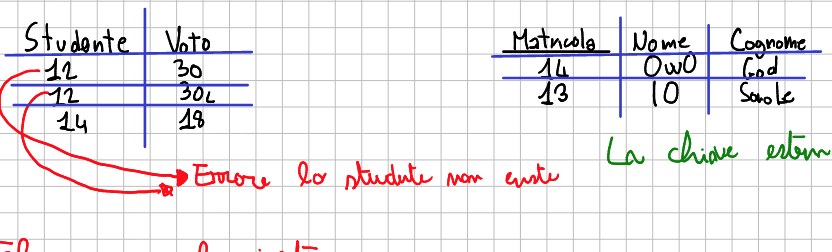
\includegraphics[width=\textwidth]{img/chiave_esterna.png}

\subsection{Eliminazione di chiavi esterne}

L'eliminazione di chiavi esterne è una situazione molto pericolosa e piena di insidie, va quindi eseguita con cura per mantenere l'integrità del dominio che si sta rappresentando nella base dati.

Le modalità di eliminazione di dati inseriti nel contesto delle chiavi esterne sono di vari tipi:

\begin{itemize}
    \item On delete cascade, ovvero elimino tutti i dati che utilizzano la chiave esterna.
    \item Assegnazione di \textit{NULL}
    \item Errore di eliminazione, ovvero devo prima eliminare manualmente i dati che utilizzano la chiave esterna.
\end{itemize}

\section{Super-chiavi}

Le super-chiavi permettono di capire di quale riga stiamo parlando. Sarà importante che una riga sia sempre super-chiave, questo determina infatti la non ridondanza dei dati nella tabella.

\begin{description}
	\item[N.B.] Più la super-chiave è piccola, e interessa quindi meno campi, meglio è, infatti più la super-chiave è piccola più è ampio l'insieme di dati che possiamo salvare.
\end{description}